% !TeX TXS-program:compile = txs:///pdflatex/[--shell-escape]
%%%%%%%%%%%%%%%%%%%%%%%%%%%%%%%%%%%%%%%%%
% The Legrand Orange Book
% LaTeX Template
% Version 2.1.1 (14/2/16)
%
% This template has been downloaded from:
% http://www.LaTeXTemplates.com
%
% Original author:
% Mathias Legrand (legrand.mathias@gmail.com) with modifications by:
% Vel (vel@latextemplates.com)
%
% License:
% CC BY-NC-SA 3.0 (http://creativecommons.org/licenses/by-nc-sa/3.0/)
%
% Compiling this template:
% This template uses biber for its bibliography and makeindex for its index.
% When you first open the template, compile it from the command line with the 
% commands below to make sure your LaTeX distribution is configured correctly:
%
% 1) pdflatex main
% 2) makeindex main.idx -s StyleInd.ist
% 3) biber main
% 4) pdflatex main x 2
%
% After this, when you wish to update the bibliography/index use the appropriate
% command above and make sure to compile with pdflatex several times 
% afterwards to propagate your changes to the document.
%
% This template also uses a number of packages which may need to be
% updated to the newest versions for the template to compile. It is strongly
% recommended you update your LaTeX distribution if you have any
% compilation errors.
%
% Important note:
% Chapter heading images should have a 2:1 width:height ratio,
% e.g. 920px width and 460px height.
%
%%%%%%%%%%%%%%%%%%%%%%%%%%%%%%%%%%%%%%%%%

%----------------------------------------------------------------------------------------
%	PACKAGES AND OTHER DOCUMENT CONFIGURATIONS
%----------------------------------------------------------------------------------------

\documentclass[11pt,fleqn]{book} % Default font size and left-justified equations

%----------------------------------------------------------------------------------------

%%%%%%%%%%%%%%%%%%%%%%%%%%%%%%%%%%%%%%%%%
% The Legrand Orange Book
% Structural Definitions File
% Version 2.0 (9/2/15)
%
% Original author:
% Mathias Legrand (legrand.mathias@gmail.com) with modifications by:
% Vel (vel@latextemplates.com)
% 
% This file has been downloaded from:
% http://www.LaTeXTemplates.com
%
% License:
% CC BY-NC-SA 3.0 (http://creativecommons.org/licenses/by-nc-sa/3.0/)
%
%%%%%%%%%%%%%%%%%%%%%%%%%%%%%%%%%%%%%%%%%

%----------------------------------------------------------------------------------------
%	VARIOUS REQUIRED PACKAGES AND CONFIGURATIONS
%----------------------------------------------------------------------------------------

\usepackage[top=3cm,bottom=3cm,left=3cm,right=3cm,headsep=10pt,a4paper]{geometry} % Page margins

\usepackage{graphicx} % Required for including pictures
\graphicspath{{Pictures/}} % Specifies the directory where pictures are stored

\usepackage{lipsum} % Inserts dummy text

\usepackage{tikz} % Required for drawing custom shapes

\usepackage[english]{babel} % English language/hyphenation

\usepackage{enumitem} % Customize lists
\setlist{nolistsep} % Reduce spacing between bullet points and numbered lists

\usepackage{booktabs} % Required for nicer horizontal rules in tables

\usepackage{xcolor} % Required for specifying colors by name
\definecolor{ocre}{RGB}{243,102,25} % Define the orange color used for highlighting throughout the book
\usepackage{minted} % Required to display colored code properly
%hack for minted to get rid of syntax error boxes
\makeatletter
\AtBeginEnvironment{minted}{\dontdofcolorbox}
\def\dontdofcolorbox{\renewcommand\fcolorbox[4][]{##4}}
\makeatother



\usepackage{wrapfig} % Required to display wrapped figures with text

\usepackage{subcaption} %Required to allow subfigures

\usepackage{adjustbox} %Required for proper alignment of minipages

\newcommand{\chref}[3][blue]{\href{#2}{\color{#1}{#3}}}%

%----------------------------------------------------------------------------------------
%	FONTS
%----------------------------------------------------------------------------------------

\usepackage{avant} % Use the Avantgarde font for headings
%\usepackage{times} % Use the Times font for headings
\usepackage{mathptmx} % Use the Adobe Times Roman as the default text font together with math symbols from the Sym­bol, Chancery and Com­puter Modern fonts

\usepackage{microtype} % Slightly tweak font spacing for aesthetics
\usepackage[utf8]{inputenc} % Required for including letters with accents
\usepackage[T1]{fontenc} % Use 8-bit encoding that has 256 glyphs

%----------------------------------------------------------------------------------------
%	BIBLIOGRAPHY AND INDEX
%----------------------------------------------------------------------------------------

\usepackage[style=alphabetic,citestyle=numeric,sorting=nyt,sortcites=true,autopunct=true,babel=hyphen,hyperref=true,abbreviate=false,backref=true,backend=biber]{biblatex}
\addbibresource{bibliography.bib} % BibTeX bibliography file
\defbibheading{bibempty}{}

\usepackage{calc} % For simpler calculation - used for spacing the index letter headings correctly
\usepackage{makeidx} % Required to make an index
\makeindex % Tells LaTeX to create the files required for indexing

%----------------------------------------------------------------------------------------
%	MAIN TABLE OF CONTENTS
%----------------------------------------------------------------------------------------

\usepackage{titletoc} % Required for manipulating the table of contents

\contentsmargin{0cm} % Removes the default margin

% Part text styling
\titlecontents{part}[0cm]
{\addvspace{20pt}\centering\large\bfseries}
{}
{}
{}

% Chapter text styling
\titlecontents{chapter}[1.25cm] % Indentation
{\addvspace{12pt}\large\sffamily\bfseries} % Spacing and font options for chapters
{\color{ocre!60}\contentslabel[\Large\thecontentslabel]{1.25cm}\color{ocre}} % Chapter number
{\color{ocre}}  
{\color{ocre!60}\normalsize\;\titlerule*[.5pc]{.}\;\thecontentspage} % Page number

% Section text styling
\titlecontents{section}[1.25cm] % Indentation
{\addvspace{3pt}\sffamily\bfseries} % Spacing and font options for sections
{\contentslabel[\thecontentslabel]{1.25cm}} % Section number
{}
{\hfill\color{black}\thecontentspage} % Page number
[]

% Subsection text styling
\titlecontents{subsection}[1.25cm] % Indentation
{\addvspace{1pt}\sffamily\small} % Spacing and font options for subsections
{\contentslabel[\thecontentslabel]{1.25cm}} % Subsection number
{}
{\ \titlerule*[.5pc]{.}\;\thecontentspage} % Page number
[]

% List of figures
\titlecontents{figure}[0em]
{\addvspace{-5pt}\sffamily}
{\thecontentslabel\hspace*{1em}}
{}
{\ \titlerule*[.5pc]{.}\;\thecontentspage}
[]

% List of tables
\titlecontents{table}[0em]
{\addvspace{-5pt}\sffamily}
{\thecontentslabel\hspace*{1em}}
{}
{\ \titlerule*[.5pc]{.}\;\thecontentspage}
[]

%----------------------------------------------------------------------------------------
%	MINI TABLE OF CONTENTS IN PART HEADS
%----------------------------------------------------------------------------------------

% Chapter text styling
\titlecontents{lchapter}[0em] % Indenting
{\addvspace{15pt}\large\sffamily\bfseries} % Spacing and font options for chapters
{\color{ocre}\contentslabel[\Large\thecontentslabel]{1.25cm}\color{ocre}} % Chapter number
{}  
{\color{ocre}\normalsize\sffamily\bfseries\;\titlerule*[.5pc]{.}\;\thecontentspage} % Page number

% Section text styling
\titlecontents{lsection}[0em] % Indenting
{\sffamily\small} % Spacing and font options for sections
{\contentslabel[\thecontentslabel]{1.25cm}} % Section number
{}
{}

% Subsection text styling
\titlecontents{lsubsection}[.5em] % Indentation
{\normalfont\footnotesize\sffamily} % Font settings
{}
{}
{}

%----------------------------------------------------------------------------------------
%	PAGE HEADERS
%----------------------------------------------------------------------------------------

\usepackage{fancyhdr} % Required for header and footer configuration

\pagestyle{fancy}
\renewcommand{\chaptermark}[1]{\markboth{\sffamily\normalsize\bfseries\chaptername\ \thechapter.\ #1}{}} % Chapter text font settings
\renewcommand{\sectionmark}[1]{\markright{\sffamily\normalsize\thesection\hspace{5pt}#1}{}} % Section text font settings
\fancyhf{} \fancyhead[LE,RO]{\sffamily\normalsize\thepage} % Font setting for the page number in the header
\fancyhead[LO]{\rightmark} % Print the nearest section name on the left side of odd pages
\fancyhead[RE]{\leftmark} % Print the current chapter name on the right side of even pages
\renewcommand{\headrulewidth}{0.5pt} % Width of the rule under the header
\addtolength{\headheight}{2.5pt} % Increase the spacing around the header slightly
\renewcommand{\footrulewidth}{0pt} % Removes the rule in the footer
\fancypagestyle{plain}{\fancyhead{}\renewcommand{\headrulewidth}{0pt}} % Style for when a plain pagestyle is specified

% Removes the header from odd empty pages at the end of chapters
\makeatletter
\renewcommand{\cleardoublepage}{
\clearpage\ifodd\c@page\else
\hbox{}
\vspace*{\fill}
\thispagestyle{empty}
\newpage
\fi}

%----------------------------------------------------------------------------------------
%	THEOREM STYLES
%----------------------------------------------------------------------------------------

\usepackage{amsmath,amsfonts,amssymb,amsthm} % For math equations, theorems, symbols, etc

\newcommand{\intoo}[2]{\mathopen{]}#1\,;#2\mathclose{[}}
\newcommand{\ud}{\mathop{\mathrm{{}d}}\mathopen{}}
\newcommand{\intff}[2]{\mathopen{[}#1\,;#2\mathclose{]}}
\newtheorem{notation}{Notation}[chapter]

% Boxed/framed environments
\newtheoremstyle{ocrenumbox}% % Theorem style name
{0pt}% Space above
{0pt}% Space below
{\normalfont}% % Body font
{}% Indent amount
{\small\bf\sffamily\color{ocre}}% % Theorem head font
{\;}% Punctuation after theorem head
{0.25em}% Space after theorem head
{\small\sffamily\color{ocre}\thmname{#1}\nobreakspace\thmnumber{\@ifnotempty{#1}{}\@upn{#2}}% Theorem text (e.g. Theorem 2.1)
\thmnote{\nobreakspace\the\thm@notefont\sffamily\bfseries\color{black}---\nobreakspace#3.}} % Optional theorem note
\renewcommand{\qedsymbol}{$\blacksquare$}% Optional qed square

\newtheoremstyle{blacknumex}% Theorem style name
{5pt}% Space above
{5pt}% Space below
{\normalfont}% Body font
{} % Indent amount
{\small\bf\sffamily}% Theorem head font
{\;}% Punctuation after theorem head
{0.25em}% Space after theorem head
{\small\sffamily{\tiny\ensuremath{\blacksquare}}\nobreakspace\thmname{#1}\nobreakspace\thmnumber{\@ifnotempty{#1}{}\@upn{#2}}% Theorem text (e.g. Theorem 2.1)
\thmnote{\nobreakspace\the\thm@notefont\sffamily\bfseries---\nobreakspace#3.}}% Optional theorem note

\newtheoremstyle{blacknumbox} % Theorem style name
{0pt}% Space above
{0pt}% Space below
{\normalfont}% Body font
{}% Indent amount
{\small\bf\sffamily}% Theorem head font
{\;}% Punctuation after theorem head
{0.25em}% Space after theorem head
{\small\sffamily\thmname{#1}\nobreakspace\thmnumber{\@ifnotempty{#1}{}\@upn{#2}}% Theorem text (e.g. Theorem 2.1)
\thmnote{\nobreakspace\the\thm@notefont\sffamily\bfseries---\nobreakspace#3.}}% Optional theorem note

% Non-boxed/non-framed environments
\newtheoremstyle{ocrenum}% % Theorem style name
{5pt}% Space above
{5pt}% Space below
{\normalfont}% % Body font
{}% Indent amount
{\small\bf\sffamily\color{ocre}}% % Theorem head font
{\;}% Punctuation after theorem head
{0.25em}% Space after theorem head
{\small\sffamily\color{ocre}\thmname{#1}\nobreakspace\thmnumber{\@ifnotempty{#1}{}\@upn{#2}}% Theorem text (e.g. Theorem 2.1)
\thmnote{\nobreakspace\the\thm@notefont\sffamily\bfseries\color{black}---\nobreakspace#3.}} % Optional theorem note
\renewcommand{\qedsymbol}{$\blacksquare$}% Optional qed square
\makeatother

% Defines the theorem text style for each type of theorem to one of the three styles above
\newcounter{dummy} 
\numberwithin{dummy}{section}
\theoremstyle{ocrenumbox}
\newtheorem{theoremeT}[dummy]{Theorem}
\newtheorem{problem}{Problem}[chapter]
\newtheorem{exerciseT}{Exercise}[chapter]
\theoremstyle{blacknumex}
\newtheorem{exampleT}{Example}[chapter]
\theoremstyle{blacknumbox}
\newtheorem{vocabulary}{Vocabulary}[chapter]
\newtheorem{definitionT}{Definition}[section]
\newtheorem{corollaryT}[dummy]{Corollary}
\theoremstyle{ocrenum}
\newtheorem{proposition}[dummy]{Proposition}

%----------------------------------------------------------------------------------------
%	DEFINITION OF COLORED BOXES
%----------------------------------------------------------------------------------------

\RequirePackage[framemethod=default]{mdframed} % Required for creating the theorem, definition, exercise and corollary boxes

% Theorem box
\newmdenv[skipabove=7pt,
skipbelow=7pt,
backgroundcolor=black!5,
linecolor=ocre,
innerleftmargin=5pt,
innerrightmargin=5pt,
innertopmargin=5pt,
leftmargin=0cm,
rightmargin=0cm,
innerbottommargin=5pt]{tBox}

% Exercise box	  
\newmdenv[skipabove=7pt,
skipbelow=7pt,
rightline=false,
leftline=true,
topline=false,
bottomline=false,
backgroundcolor=ocre!10,
linecolor=ocre,
innerleftmargin=5pt,
innerrightmargin=5pt,
innertopmargin=5pt,
innerbottommargin=5pt,
leftmargin=0cm,
rightmargin=0cm,
linewidth=4pt]{eBox}	

% Definition box
\newmdenv[skipabove=7pt,
skipbelow=7pt,
rightline=false,
leftline=true,
topline=false,
bottomline=false,
linecolor=ocre,
innerleftmargin=5pt,
innerrightmargin=5pt,
innertopmargin=0pt,
leftmargin=0cm,
rightmargin=0cm,
linewidth=4pt,
innerbottommargin=0pt]{dBox}	

% Corollary box
\newmdenv[skipabove=7pt,
skipbelow=7pt,
rightline=false,
leftline=true,
topline=false,
bottomline=false,
linecolor=gray,
backgroundcolor=black!5,
innerleftmargin=5pt,
innerrightmargin=5pt,
innertopmargin=5pt,
leftmargin=0cm,
rightmargin=0cm,
linewidth=4pt,
innerbottommargin=5pt]{cBox}

% Creates an environment for each type of theorem and assigns it a theorem text style from the "Theorem Styles" section above and a colored box from above
\newenvironment{theorem}{\begin{tBox}\begin{theoremeT}}{\end{theoremeT}\end{tBox}}
\newenvironment{exercise}{\begin{eBox}\begin{exerciseT}}{\hfill{\color{ocre}\tiny\ensuremath{\blacksquare}}\end{exerciseT}\end{eBox}}				  
\newenvironment{definition}{\begin{dBox}\begin{definitionT}}{\end{definitionT}\end{dBox}}	
\newenvironment{example}{\begin{exampleT}}{\hfill{\tiny\ensuremath{\blacksquare}}\end{exampleT}}		
\newenvironment{corollary}{\begin{cBox}\begin{corollaryT}}{\end{corollaryT}\end{cBox}}	

%----------------------------------------------------------------------------------------
%	REMARK ENVIRONMENT
%----------------------------------------------------------------------------------------

\newenvironment{remark}{\par\vspace{10pt}\small % Vertical white space above the remark and smaller font size
\begin{list}{}{
\leftmargin=35pt % Indentation on the left
\rightmargin=25pt}\item\ignorespaces % Indentation on the right
\makebox[-2.5pt]{\begin{tikzpicture}[overlay]
\node[draw=ocre!60,line width=1pt,circle,fill=ocre!25,font=\sffamily\bfseries,inner sep=2pt,outer sep=0pt] at (-15pt,0pt){\textcolor{ocre}{R}};\end{tikzpicture}} % Orange R in a circle
\advance\baselineskip -1pt}{\end{list}\vskip5pt} % Tighter line spacing and white space after remark

%----------------------------------------------------------------------------------------
%	SECTION NUMBERING IN THE MARGIN
%----------------------------------------------------------------------------------------

\makeatletter
\renewcommand{\@seccntformat}[1]{\llap{\textcolor{ocre}{\csname the#1\endcsname}\hspace{1em}}}                    
\renewcommand{\section}{\@startsection{section}{1}{\z@}
{-4ex \@plus -1ex \@minus -.4ex}
{1ex \@plus.2ex }
{\normalfont\large\sffamily\bfseries}}
\renewcommand{\subsection}{\@startsection {subsection}{2}{\z@}
{-3ex \@plus -0.1ex \@minus -.4ex}
{0.5ex \@plus.2ex }
{\normalfont\sffamily\bfseries}}
\renewcommand{\subsubsection}{\@startsection {subsubsection}{3}{\z@}
{-2ex \@plus -0.1ex \@minus -.2ex}
{.2ex \@plus.2ex }
{\normalfont\small\sffamily\bfseries}}                        
\renewcommand\paragraph{\@startsection{paragraph}{4}{\z@}
{-2ex \@plus-.2ex \@minus .2ex}
{.1ex}
{\normalfont\small\sffamily\bfseries}}

%----------------------------------------------------------------------------------------
%	PART HEADINGS
%----------------------------------------------------------------------------------------

% numbered part in the table of contents
\newcommand{\@mypartnumtocformat}[2]{%
\setlength\fboxsep{0pt}%
\noindent\colorbox{ocre!20}{\strut\parbox[c][.7cm]{\ecart}{\color{ocre!70}\Large\sffamily\bfseries\centering#1}}\hskip\esp\colorbox{ocre!40}{\strut\parbox[c][.7cm]{\linewidth-\ecart-\esp}{\Large\sffamily\centering#2}}}%
%%%%%%%%%%%%%%%%%%%%%%%%%%%%%%%%%%
% unnumbered part in the table of contents
\newcommand{\@myparttocformat}[1]{%
\setlength\fboxsep{0pt}%
\noindent\colorbox{ocre!40}{\strut\parbox[c][.7cm]{\linewidth}{\Large\sffamily\centering#1}}}%
%%%%%%%%%%%%%%%%%%%%%%%%%%%%%%%%%%
\newlength\esp
\setlength\esp{4pt}
\newlength\ecart
\setlength\ecart{1.2cm-\esp}
\newcommand{\thepartimage}{}%
\newcommand{\partimage}[1]{\renewcommand{\thepartimage}{#1}}%
\def\@part[#1]#2{%
\ifnum \c@secnumdepth >-2\relax%
\refstepcounter{part}%
\addcontentsline{toc}{part}{\texorpdfstring{\protect\@mypartnumtocformat{\thepart}{#1}}{\partname~\thepart\ ---\ #1}}
\else%
\addcontentsline{toc}{part}{\texorpdfstring{\protect\@myparttocformat{#1}}{#1}}%
\fi%
\startcontents%
\markboth{}{}%
{\thispagestyle{empty}%
\begin{tikzpicture}[remember picture,overlay]%
\node at (current page.north west){\begin{tikzpicture}[remember picture,overlay]%	
\fill[ocre!30](0cm,0cm) rectangle (\paperwidth,-\paperheight);
\node[anchor=north west] at (0.5cm,-3.25cm){\color{black!80}\fontsize{150}{100}\sffamily\bfseries\@Roman\c@part}; 
\node[anchor=south east] at (\paperwidth-1cm,-\paperheight+1cm){\parbox[t][][t]{8.5cm}{
\printcontents{l}{0}{\setcounter{tocdepth}{1}}%
}};
\node[anchor=north east] at (\paperwidth-1.5cm,-3.25cm){\parbox[t][][t]{15cm}{\strut\raggedleft\color{blue}\fontsize{30}{30}\sffamily\bfseries#2}};
\end{tikzpicture}};
\end{tikzpicture}}%
\@endpart}
\def\@spart#1{%
\startcontents%
\phantomsection
{\thispagestyle{empty}%
\begin{tikzpicture}[remember picture,overlay]%
\node at (current page.north west){\begin{tikzpicture}[remember picture,overlay]%	
\fill[ocre!20](0cm,0cm) rectangle (\paperwidth,-\paperheight);
\node[anchor=north east] at (\paperwidth-1.5cm,-3.25cm){\parbox[t][][t]{15cm}{\strut\raggedleft\color{white}\fontsize{30}{30}\sffamily\bfseries#1}};
\end{tikzpicture}};
\end{tikzpicture}}
\addcontentsline{toc}{part}{\texorpdfstring{%
\setlength\fboxsep{0pt}%
\noindent\protect\colorbox{ocre!40}{\strut\protect\parbox[c][.7cm]{\linewidth}{\Large\sffamily\protect\centering #1\quad\mbox{}}}}{#1}}%
\@endpart}
\def\@endpart{\vfil\newpage
\if@twoside
\if@openright
\null
\thispagestyle{empty}%
\newpage
\fi
\fi
\if@tempswa
\twocolumn
\fi}

%----------------------------------------------------------------------------------------
%	CHAPTER HEADINGS
%----------------------------------------------------------------------------------------

% A switch to conditionally include a picture, implemented by  Christian Hupfer
\newif\ifusechapterimage
\usechapterimagetrue
\newcommand{\thechapterimage}{}%
\newcommand{\chapterimage}[1]{\ifusechapterimage\renewcommand{\thechapterimage}{#1}\fi}%
\def\@makechapterhead#1{%
{\parindent \z@ \raggedright \normalfont
\ifnum \c@secnumdepth >\m@ne
\if@mainmatter
\begin{tikzpicture}[remember picture,overlay]
\node at (current page.north west)
{\begin{tikzpicture}[remember picture,overlay]
\node[anchor=north west,inner sep=0pt] at (0,0) {\ifusechapterimage\includegraphics[width=\paperwidth]{\thechapterimage}\fi};
\draw[anchor=west] (\Gm@lmargin,-9cm) node [line width=2pt,rounded corners=15pt,draw=ocre,fill=white,fill opacity=0.5,inner sep=15pt]{\strut\makebox[22cm]{}};
\draw[anchor=west] (\Gm@lmargin+.3cm,-9cm) node {\huge\sffamily\bfseries\color{black}\thechapter. #1\strut};
\end{tikzpicture}};
\end{tikzpicture}
\else
\begin{tikzpicture}[remember picture,overlay]
\node at (current page.north west)
{\begin{tikzpicture}[remember picture,overlay]
\node[anchor=north west,inner sep=0pt] at (0,0) {\ifusechapterimage\includegraphics[width=\paperwidth]{\thechapterimage}\fi};
\draw[anchor=west] (\Gm@lmargin,-9cm) node [line width=2pt,rounded corners=15pt,draw=ocre,fill=white,fill opacity=0.5,inner sep=15pt]{\strut\makebox[22cm]{}};
\draw[anchor=west] (\Gm@lmargin+.3cm,-9cm) node {\huge\sffamily\bfseries\color{black}#1\strut};
\end{tikzpicture}};
\end{tikzpicture}
\fi\fi\par\vspace*{270\p@}}}

%-------------------------------------------

\def\@makeschapterhead#1{%
\begin{tikzpicture}[remember picture,overlay]
\node at (current page.north west)
{\begin{tikzpicture}[remember picture,overlay]
\node[anchor=north west,inner sep=0pt] at (0,0) {\ifusechapterimage\includegraphics[width=\paperwidth]{\thechapterimage}\fi};
\draw[anchor=west] (\Gm@lmargin,-9cm) node [line width=2pt,rounded corners=15pt,draw=ocre,fill=white,fill opacity=0.5,inner sep=15pt]{\strut\makebox[22cm]{}};
\draw[anchor=west] (\Gm@lmargin+.3cm,-9cm) node {\huge\sffamily\bfseries\color{black}#1\strut};
\end{tikzpicture}};
\end{tikzpicture}
\par\vspace*{270\p@}}
\makeatother

%----------------------------------------------------------------------------------------
%	HYPERLINKS IN THE DOCUMENTS
%----------------------------------------------------------------------------------------

\usepackage{hyperref}
\hypersetup{hidelinks,backref=true,pagebackref=true,hyperindex=true,colorlinks=false,breaklinks=true,urlcolor= ocre,bookmarks=true,bookmarksopen=false,pdftitle={Title},pdfauthor={Author}}
\usepackage{bookmark}
\bookmarksetup{
open,
numbered,
addtohook={%
\ifnum\bookmarkget{level}=0 % chapter
\bookmarksetup{bold}%
\fi
\ifnum\bookmarkget{level}=-1 % part
\bookmarksetup{color=ocre,bold}%
\fi
}
}
 % Insert the commands.tex file which contains the majority of the structure behind the template

\begin{document}

%----------------------------------------------------------------------------------------
%	TITLE PAGE
%----------------------------------------------------------------------------------------

\begingroup
\thispagestyle{empty}
\begin{tikzpicture}[remember picture,overlay]
\coordinate [below=8cm] (midpoint) at (current page.north);
\node at (current page.north west)
{\begin{tikzpicture}[remember picture,overlay]
\node[anchor=north west,inner sep=0pt] at (0,0) {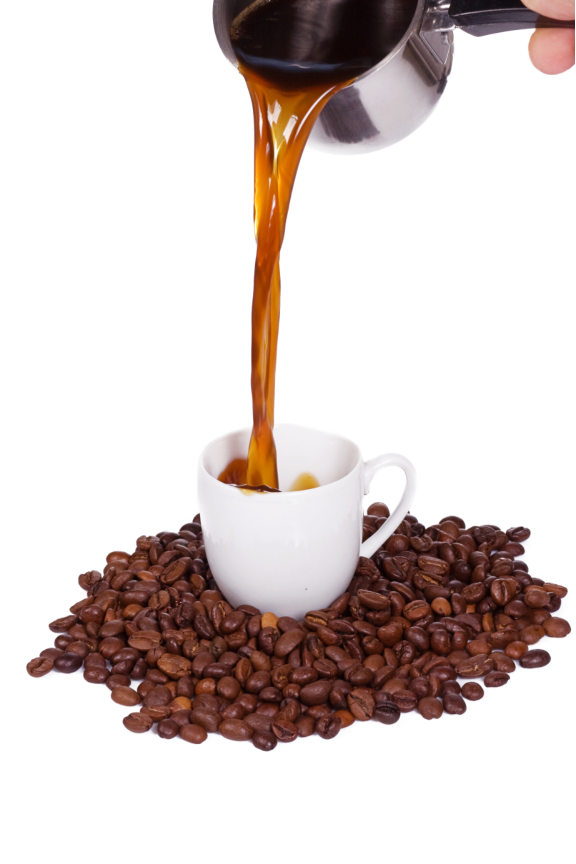
\includegraphics[width=\paperwidth]{Kaffe.pdf}}; % Background image
\draw[anchor=north] (midpoint) node [fill=ocre!30!white,fill opacity=0.8,text opacity=1,inner sep=1cm]{\Huge\centering\bfseries\sffamily\parbox[c][][t]{\paperwidth}{\centering DFiant Hardware Description Language\\[15pt] % Book title
{\Large Design By Example}\\[20pt] % Subtitle
{\huge Oron Port}}}; % Author name
\end{tikzpicture}};
\end{tikzpicture}
\vfill
\endgroup

%----------------------------------------------------------------------------------------
%	COPYRIGHT PAGE
%----------------------------------------------------------------------------------------

\newpage
~\vfill
\thispagestyle{empty}

\noindent Copyright \copyright\ 2015 Oron Port\\ % Copyright notice

%\noindent \textsc{Published by Publisher}\\ % Publisher

%\noindent \textsc{book-website.com}\\ % URL

\noindent Licensed under the Creative Commons Attribution-NonCommercial 3.0 Unported License (the ``License''). You may not use this file except in compliance with the License. You may obtain a copy of the License at \url{http://creativecommons.org/licenses/by-nc/3.0}. Unless required by applicable law or agreed to in writing, software distributed under the License is distributed on an \textsc{``as is'' basis, without warranties or conditions of any kind}, either express or implied. See the License for the specific language governing permissions and limitations under the License.\\ % License information

%\noindent \textit{First printing, March 2013} % Printing/edition date

%----------------------------------------------------------------------------------------
%	TABLE OF CONTENTS
%----------------------------------------------------------------------------------------

%\usechapterimagefalse % If you don't want to include a chapter image, use this to toggle images off - it can be enabled later with \usechapterimagetrue

\chapterimage{chapter_head_1.pdf} % Table of contents heading image

\pagestyle{empty} % No headers

\tableofcontents % Print the table of contents itself

\cleardoublepage % Forces the first chapter to start on an odd page so it's on the right

\pagestyle{fancy} % Print headers again

%----------------------------------------------------------------------------------------
%	PART
%----------------------------------------------------------------------------------------

\part{Introduction}

%----------------------------------------------------------------------------------------
%	PART
%----------------------------------------------------------------------------------------
\part{Basic Syntax}

\chapterimage{chapter_head_2.pdf} % Chapter heading image
\chapter{DFiant Syntax}

\section{DFiant as a Scala library}
DFiant is a Scala library and creates its own DSL (Domain Specific Language) within Scala's syntax boundaries. DFiant extends Scala by creating its own classes, types, definition, operators, etc. Therefore, all Scala code is a valid DFiant code, as long as it does not interact with DFiant-exclusive code. Of course this will not result in any runtime DFiant produce, but will pass compilation nonetheless. DFiant requires no special parser, allowing Scala IDE's and tools to be used for DFiant code development, debugging and deployment.\\

The following table is a summary of errors and their trapping mechanisms:\\
\begin{tabular}{||c|c|c||}
	\hline 
	Error Level & Trapping Mechanism 				& Typical errors \\ 
	\hline 
	1 					& IDE Error Highlighting 		& Type safety, DFMutability safety \\ 
	\hline 
	2 					& Scala Compilation Error 	& Type safety, DFMutability safety \\ 
	\hline 
	3 					& DFiant Compiler Error 
	              (Scala Runtime Exception) & TBD \\ 
	\hline 
	4 					& DFiant Simulator Error 
	              (Scala Runtime Exception) & TBD \\ 
	\hline 
\end{tabular} \\
\vfill
\newpage

The following table contains references to chapters of the \chref{http://www.scala-lang.org/files/archive/spec/2.11/}{Scala Language Specification}. Some chapters were extended in DFiant, but most remain unmodified.\\
\begin{tabular}{||c|c|p{8cm}||}
	\hline 
	Chapter 		& Title 				& DFiant Extension \\ 
	\hline 
	1 & \chref{http://www.scala-lang.org/files/archive/spec/2.11/01-lexical-syntax.html}{Lexical Syntax}	& Unmodified \\ 
	\hline 
	2 & \chref{http://www.scala-lang.org/files/archive/spec/2.11/02-identifiers-names-and-scopes.html}{Identifiers, Names and Scopes} & Unmodified \\
	\hline 
	3 & \chref{http://www.scala-lang.org/files/archive/spec/2.11/03-types.html}{Types} & Unmodified \\
	\hline 
	4 & \chref{http://www.scala-lang.org/files/archive/spec/2.11/04-basic-declarations-and-definitions.html}{Basic Declarations and Definitions} & 
	Mutable dataflow stream variables. \newline 
	Immutable dataflow stream values. \newline 
	Bit selection \& casting \newline
	Temporal Past \& Future token access. \\
	\hline 
	5 & \chref{http://www.scala-lang.org/files/archive/spec/2.11/05-classes-and-objects.html}{Classes and Objects} & 
	Structural IN/OUT abstract representation \\
	\hline 
	6 & \chref{http://www.scala-lang.org/files/archive/spec/2.11/06-expressions.html}{Expressions} & 
	Dataflow 'If' expression \newline
	Design 'If' expression \newline
	Token temporal consumption \& production control \\
	\hline 
	7 & \chref{http://www.scala-lang.org/files/archive/spec/2.11/07-implicits.html}{Implicit} & Unmodified \\
	\hline 
	8 & \chref{http://www.scala-lang.org/files/archive/spec/2.11/08-pattern-matching.html}{Pattern Matching} & Unmodified \\
	\hline 
	9 & \chref{http://www.scala-lang.org/files/archive/spec/2.11/09-top-level-definitions.html}{Top-Level Definitions} & Unmodified \\
	\hline 
	10 & \chref{http://www.scala-lang.org/files/archive/spec/2.11/10-xml-expressions-and-patterns.html}{XML Expressions and Patterns} & Unmodified \\
	\hline 
	11 & \chref{http://www.scala-lang.org/files/archive/spec/2.11/11-annotations.html}{Annotations} & 
	DFiant Compiler Annotations \newline
	Solution Constraints \\
	\hline 
	12 & \chref{http://www.scala-lang.org/files/archive/spec/2.11/12-the-scala-standard-library.html}{The Scala Standard Library} & The DFiant Standard Library \newline
	Basic Library \\
	\hline 
	13 & \chref{http://www.scala-lang.org/files/archive/spec/2.11/13-syntax-summary.html}{Syntax Summary} & Extended by DFiant \\
	\hline 
\end{tabular} \\



\begin{minted}[tabsize=2,gobble=1,framesep=5pt]{bnf}
	UnicodeEscape ::= ‘\’ ‘u’ {‘u’} hexDigit hexDigit hexDigit hexDigit
	hexDigit      ::= ‘0’ | … | ‘9’ | ‘A’ | … | ‘F’ | ‘a’ | … | ‘f’
\end{minted}


%----------------------------------------------------------------------------------------
%	PART
%----------------------------------------------------------------------------------------
\part{Scheduling}

%----------------------------------------------------------------------------------------
%	Dataflow definition convention
%----------------------------------------------------------------------------------------
\chapterimage{chapter_head_2.pdf} % Chapter heading image
\chapter{Dataflow definition convention}
To define required dataflow functionality, we naturally use sequences to describe inputs/outputs to/from a function. We assume the sequences to be finite.\footnote{Our dataflow is used to describe hardware. Eventually all hardware stops working :-)} 

\begin{definition}[Dataflow sequence]
	A dataflow sequence of a variable $var$ at length of $N$ is defined as follows:
	\begin{equation}
		S_{var}^{N}\triangleq \left( var_0,var_1,\cdots,var_N \right)
	\end{equation}
\end{definition}

\begin{definition}[Dataflow sequence set]
	A dataflow sequence set $SS_{DF}$ is a set of finite dataflow sequences and is defined as follows:
	\begin{equation}
		SS_{DF}\triangleq \left\lbrace{S_{var_A}^{N_A}, S_{var_B}^{N_B},\cdots}\right\rbrace
	\end{equation}
\end{definition}

\begin{definition}[Dataflow function]
	A dataflow function $f_{DF}:SS_{DF,in}\rightarrow SS_{DF,out}$ defines the relation between the input sequence set $SS_{DF,in}$ and the output sequence set $SS_{DF,out}$. Each function is definable as follows:
	\begin{equation}
		SS_{DF,out}=f_{DF}\left(SS_{DF,in} \right) 
	\end{equation}
	\begin{remark}
		If there is a condition at which an output is not defined by the function, then the output is invalid at that condition, thus the function does not fire and no output will be produced at that condition.
	\end{remark}
\end{definition}

\begin{definition}[Dataflow Single Input, Single Output (SISO) function]
	A dataflow SISO function has a single input sequence and a single output sequence.
	\begin{corollary}
		A dataflow SISO function may consume at most a single token at any given time and produce a single token at any given time.
	\end{corollary}

	\begin{notation}
		Any dataflow function may be described as follows:
		\begin{equation*}
			\left( out_0,out_1,\cdots,out_T \right)=f\left( in_0,in_1,\cdots,in_N \right)
		\end{equation*}
	\end{notation}

	\begin{notation}
		We will usually use a shorthand approach:
		\begin{equation*}
			out_t = \begin{cases}
				h_1(in_{t}, t) & condition_1 \\
				h_2(in_{t}, t) & condition_2 \\
				\vdots & \vdots
			\end{cases}
		\end{equation*}
		If none of the conditions is matched, the function is invalid and will not fire (no token is produced).
	\end{notation}
	
\end{definition}
%----------------------------------------------------------------------------------------




%----------------------------------------------------------------------------------------
%	Dataflow definition convention
%----------------------------------------------------------------------------------------
\chapter{Scheduling Syntax}
\section{DF implicit consumption \& production}
Most DF scheduling in DFiant is implicit. The default scheduling behavior is detailed in this section. The behavior aims to minimize chance for deadlocks in case the designer forgets to specify the scheduling explicitly.

\subsection*{Implicit consumption of a produced token}
Every DF variable (either mutable or immutable) can produce a token. This token will always be consumed, even if not used (no read from the variable), unless specified otherwise (see TBD). 

\subsection*{Implicit production of a consumable token}
Every constructed DF mutable variable always produces the previous token value it was assigned, unless specified otherwise (see ). . This value will always be consumed, even if not used (no read from the variable), unless specified otherwise (see TBD).

\section{DF conditional consumption \& production}
\section{new <DFVar>(init) initialized constructor}
\section{<DFVar>:= assignment}
\section{<DFVar>.prev history value access}
\section{<DFVar>.prevInit initialized history value access}
\section{<DFVar>.isNotEmpty checks for a valid token at capable producer}
\section{<DFVar>.isNotFull checks for an empty slot at capable consumer}
\section{<DFVar>.next future value access}
\section{<DFVar>.dontConsume prevent value consumption}
\section{<DFVar>.dontProduce prevent value production}

%----------------------------------------------------------------------------------------




%----------------------------------------------------------------------------------------
%	Static Scheduling
%----------------------------------------------------------------------------------------
\chapter{Static Scheduling}
\section{SISO Example: Identity function}
\noindent
\adjustbox{valign=t}{\begin{minipage}{0.65\textwidth}
	\paragraph{Requirement}
	An identity function requires the output sequence to be identical in value and ordering to the input sequence. 
	\paragraph{Example}
	$myId(0,1,2,3,4,5,6) => (0,1,2,3,4,5,6)$
	\paragraph{Definition}
	\begin{equation*}
		out_t=
		myId\left(S_{in}^{N} \right)= 
		\begin{cases}
			in_{t} & t<N
		\end{cases}
	\end{equation*}
	All produced tokens are identical to the consumed tokens. An output token is valid (produced) as long as its index is smaller than the number of input (consumed) tokens. 
	\paragraph{Code}
	\begin{minted}[tabsize=2,gobble=2,framesep=5pt]{Scala}
		def myId(in : DFBits) : DFBits = {
			val out = DFBits(in.width) 
			out := in
			return out
		}
	\end{minted}
	It is possible to use Scala's less verbose approach, as the following code demonstrates. Throughout the examples of this guide we will usually choose the former approach, for consistency and to aid Scala beginner coders. 
	\paragraph{Code (less verbose)}
	\begin{minted}[tabsize=2,gobble=2,framesep=5pt]{Scala}
		def myId(in : DFBits) : DFBits =
			val out = DFBits(in.width) := in
	\end{minted}
\end{minipage}}\hfill%
\adjustbox{valign=t}{\begin{minipage}{0.3\textwidth}
	\adjincludegraphics[trim={0 0 0 {0.08\height}},clip,width=\textwidth]{sched/graphics/myId.pdf}
\end{minipage}}
\vfill
\pagebreak

\section{SISO Example: Triplet reverse ordering}
\noindent
\adjustbox{valign=t}{\begin{minipage}{0.65\textwidth}
	\paragraph{Requirement}
	Every three numbers are reversed at the output.
	
	\paragraph{Example}
	$myReverse(0,1,2,3,4,5,6) => (2,1,0,5,4,3)$\\
	Pay notice that the 7th token (value of 6) will be consumed by the function but there will not be a 7th token produced. The function would require two more input token to be able to produce an output.
	\paragraph{Definition}
	\begin{equation*}
		out_{t}=myReverse\left(S_{in}^{N} \right)= 
		\begin{cases}
			in_{t+2}        & t\;mod\;3=0,\;t<\left\lfloor N/3 \right\rfloor\cdot{3} \\
			in_{t}          & t\;mod\;3=1,\;t<\left\lfloor N/3 \right\rfloor\cdot{3} \\
			in_{t-2}        & t\;mod\;3=2,\;t<\left\lfloor N/3 \right\rfloor\cdot{3}
		\end{cases}
	\end{equation*}
	Explanation..... 
	\paragraph{Code}
	\begin{minted}[tabsize=2,gobble=2,framesep=5pt]{Scala}
		def myReverse(in : DFBits) : DFBits = {
			val out = DFBits(in.width)
			out <-- in.getNextSeq(3).reverse
			return out
		}
	\end{minted}
\end{minipage}}\hfill%
\adjustbox{valign=t}{\begin{minipage}{0.3\textwidth}
	\adjincludegraphics[trim={0 0 0 {0.08\height}},clip,width=\textwidth]{sched/graphics/myReverse.pdf}
\end{minipage}}

		
\section{SISO Example: Triplet identity function}
\noindent
\adjustbox{valign=t}{\begin{minipage}{0.65\textwidth}
	\paragraph{Requirement}
	Every three numbers are produced AS-IS at the output.
	
	\paragraph{Example}
	$myIdTriple(0,1,2,3,4,5,6,7) => (0,1,2,3,4,5)$\\
	Pay notice that the 7th and 8th tokens (values of 6 and 7) will be consumed by the function but will not be produced. 
	\paragraph{Definition}
	\begin{equation*}
		out_{t}=myIdTriple\left(S_{in}^{N} \right)= 
		\begin{cases}
			in_{t}        & t<\left\lfloor N/3 \right\rfloor\cdot{3} \\
		\end{cases}
	\end{equation*}
	\paragraph{Code}
	\begin{minted}[tabsize=2,gobble=2,framesep=5pt]{Scala}
		def myIdTriple(in : DFBits) : DFBits = {
			val out = DFBits(in.width)
			out <-- in.getNextSeq(3)
			return out
		}
	\end{minted}
	\paragraph{Remark}
	\begin{equation*}
		myReverse\left ( myReverse\left (*  \right ) \right ) \equiv myIdTriple(*)\not\equiv myId(*) 
	\end{equation*}
	
\end{minipage}}\hfill%
\adjustbox{valign=t}{\begin{minipage}{0.3\textwidth}
	\adjincludegraphics[trim={0 0 0 {0.08\height}},clip,width=\textwidth]{sched/graphics/myIdTriple.pdf}
\end{minipage}}
\vfill
\pagebreak


\section{SISO Example: Sum of three, sliding window}
\noindent
\adjustbox{valign=t}{\begin{minipage}{0.65\textwidth}
	\paragraph{Requirement}
	The output is a sliding window sum of every three consecutive inputs.
	
	\paragraph{Example}
	$mySum(0,1,2,3,4,5,6,7) => (3,6,9,12,15,18)$\\
	Pay notice that N consumed tokens will result in N-2 maximum produced tokens.
	\paragraph{Definition}
	\begin{equation*}
		out_{t}=mySum\left(S_{in}^{N} \right)= 
		\begin{cases}
			in_{t}+in_{t-1}+in_{t-2}        & 2 \leq t < N \\
		\end{cases}
	\end{equation*}
	\paragraph{Code}
	\begin{minted}[tabsize=2,gobble=2,framesep=5pt]{Scala}
		def mySum(in : DFBits) : DFBits = {
			val out = DFBits(in.width)
			out := in + in.prev + in.prev(2)
			return out
		}
	\end{minted}
	
\end{minipage}}\hfill%
\adjustbox{valign=t}{\begin{minipage}{0.3\textwidth}
	\adjincludegraphics[trim={0 0 0 {0.08\height}},clip,width=\textwidth]{sched/graphics/mySum.pdf}
\end{minipage}}


\section{SISO Example: Sum of three, sliding window, initialized}
\noindent
\adjustbox{valign=t}{\begin{minipage}{0.65\textwidth}
	\paragraph{Requirement}
	The output is a sliding window sum of every three consecutive inputs. If not enough input tokens are consumed for the first two sum procedures, the inputs are treated as zero values.
	
	\paragraph{Example}
	$mySumInit(0,1,2,3,4,5,6,7) => (0,1,3,6,9,12,15,18)$\\
	\paragraph{Definition}
	\begin{equation*}
		out_{t}=mySumInit\left(S_{in}^{N} \right)= 
		\begin{cases}
			in_{t} + 0 + 0     				& t = 0 < N \\
			in_{t}+in_{t-1} + 0        		& t = 1 < N \\
			in_{t}+in_{t-1}+in_{t-2}        & 2 \leq t < N \\
		\end{cases}
	\end{equation*}
	\paragraph{Code}
	\begin{minted}[tabsize=2,gobble=2,framesep=5pt]{Scala}
		def mySumInit(in : DFBits) : DFBits = {
			val out = DFBits(in.width)
			out := in + in.prev.init(0) + in.prev(2).init((0,0))
			return out
		}
	\end{minted}
	
\end{minipage}}\hfill%
\adjustbox{valign=t}{\begin{minipage}{0.3\textwidth}
	\adjincludegraphics[trim={0 0 0 {0.08\height}},clip,width=\textwidth]{sched/graphics/mySumInit.pdf}
\end{minipage}}
\vfill
\pagebreak

\section{SISO Example: Sum of triplet, Downsampling 3:1}
\noindent
\adjustbox{valign=t}{\begin{minipage}{0.65\textwidth}
	\paragraph{Requirement}
	The output is a downsampled sum of every triplet input. 
	
	\paragraph{Example}
	$mySumTriple(0,1,2,3,4,5,6) => (3,12)$
	\paragraph{Definition}
	\begin{equation*}
		out_{t}=mySumTriple\left(S_{in}^{N} \right)= 
		\begin{cases}
			in_{3t}+in_{3t+1}+in_{3t+2}        & t<\left\lfloor N/3 \right\rfloor \\
		\end{cases}
	\end{equation*}
	\paragraph{Code using two adders}
	\begin{minted}[tabsize=2,gobble=2,framesep=5pt]{Scala}
		def mySumTriple(in : DFBits) : DFBits = {
			val out = DFBits(in.width)
			val in_nseq = in.split(3)
			out := in_nseq(0) + in_nseq(1) + in_nseq(2)
			return out
		}
	\end{minted}
	\paragraph{Code using a single adder from library}
	\begin{minted}[tabsize=2,gobble=2,framesep=5pt]{Scala}
		import DFiant.basiclib.{Adder, Reusable}
		def mySumTriple(in : DFBits) : DFBits = {
			val adder = Reusable[Adder](in.width, in.width)
			return adder(adder(in, in.next), in.next(2))
		}
	\end{minted}
	\paragraph{Code using a single adder, do it yourself}
	\begin{minted}[tabsize=2,gobble=2,framesep=5pt]{Scala}
		import DFiant.basiclib.Adder
		case class myReusableAdder(width : Integer) {
			//TBD
		}
		def mySumTriple(in : DFBits) : DFBits = {
			val adder = myReusableAdder(in.width)
			return adder(adder(in, in.next), in.next(2))
		}
	\end{minted}
	
\end{minipage}}\hfill%
\adjustbox{valign=t}{\begin{minipage}{0.3\textwidth}
	\adjincludegraphics[trim={0 0 0 {0.08\height}},clip,width=\textwidth]{sched/graphics/mySumTriple.pdf}
\end{minipage}}
\vfill
\pagebreak




\section{SISO Example: Dual increment, Upsampling 1:3}
\noindent
\adjustbox{valign=t}{\begin{minipage}{0.65\textwidth}
	\paragraph{Requirement}
	For each input token $in$, the output will produce three tokens: $in$, $in+1$, and $in+2$. 
	
	\paragraph{Example}
	$myDualIncrement(0,3) => (0,1,2,3,4,5)$
	\paragraph{Definition}
	\begin{equation*}
		\begin{split}
		out_{t}=myDualIncrement\left(S_{in}^{N} \right)= \\
		=\begin{cases}
			in_{t/3}          & t\ mod\ 3 = 0, t < 3N\\
			in_{(t-1)/3}+1    & t\ mod\ 3 = 1, t < 3N\\
			in_{(t-2)/3}+2    & t\ mod\ 3 = 2, t < 3N\\
		\end{cases}
		\end{split}
	\end{equation*}
	\paragraph{Code using two adders}
	\begin{minted}[tabsize=2,gobble=2,framesep=5pt]{Scala}
		def myDualIncrement(in : DFBits) : DFBits = {
			val out = DFBits(in.width)
			out := in
			out.assignNext(1, in + 1)
			out.assignNext(2, in + 2)
			return out
		}
	\end{minted}
	\paragraph{Code using two adders, shorthand approach}
	\begin{minted}[tabsize=2,gobble=2,framesep=5pt]{Scala}
		def myDualIncrement(in : DFBits) : DFBits = {
			return Seq(in, in + 1, in + 2).merge(in.width)
		}
	\end{minted}
	\paragraph{Code using two incrementors}
	\begin{minted}[tabsize=2,gobble=2,framesep=5pt]{Scala}
		def myDualIncrement(in : DFBits) : DFBits = {
			val temp = in + 1
			return Seq(in, temp, temp + 1).merge(in.width)
		}
	\end{minted}
	\paragraph{Code using a single adder}
	\begin{minted}[tabsize=2,gobble=2,framesep=5pt]{Scala}
		def myDualIncrement(in : DFBits) : DFBits = {
			val adder = Reusable[Adder](in.width, in.width)
			return Seq(in, adder(in, 1), adder(in, 2)).merge(in.width)
		}
	\end{minted}
	\paragraph{Code using a single incrementor}
	\begin{minted}[tabsize=2,gobble=2,framesep=5pt]{Scala}
		def myDualIncrement(in : DFBits) : DFBits = {
			val incr = Reusable[Incrementor](in.width, 1)
			val temp = incr(in)
			return Seq(in, temp, incr(temp)).merge(in.width)
		}
	\end{minted}
	
\end{minipage}}\hfill%
\adjustbox{valign=t}{\begin{minipage}{0.3\textwidth}
	\adjincludegraphics[trim={0 0 0 {0.08\height}},clip,width=\textwidth]{sched/graphics/myDualIncrement.pdf}
\end{minipage}}
\vfill
\pagebreak


\section{SISO Example: Place first elements}
\noindent
\adjustbox{valign=t}{\begin{minipage}{0.65\textwidth}
	\paragraph{Requirement}
	Given an input and a constant sequence, the function will first output the constant sequence and then continue with the input's sequence.
		
	\paragraph{Example}
	$placeElements\left(in=(2,3,4,5,6),con=(0,1) \right)  => (0,1,2,3,4,5,6)$
	\paragraph{Definition}
	\begin{equation*}
		out_{t}=placeElements\left(S_{in}^{N}, S_{con}^{L} \right)= 
		\begin{cases}
			con_{t}      & t<L \\
			in_{t-L}     & L \leq t < N+L \\
		\end{cases}
	\end{equation*}
	\paragraph{Code}
	\begin{minted}[linenos,tabsize=2,gobble=2,framesep=5pt]{Scala}
		def placeElements(in : DFBits, con : Seq[BigInt]) 
		: DFBits = {
			val out = DFBits(in.width)
			val cnt = DFBits(Log2(con.length+1), init=0)

			ifdf (cnt == con.length) {
				out := in
			} else {
				in.dontConsume()
				out := con(cnt)
				cnt := cnt + 1
			}
			return out
		}
	\end{minted}
\end{minipage}}\hfill%
\adjustbox{valign=t}{\begin{minipage}{0.3\textwidth}
	\adjincludegraphics[trim={0 0 0 {0.08\height}},clip,width=\textwidth]{sched/graphics/placeElements.pdf}
\end{minipage}}

\paragraph{Notes}
\begin{enumerate}
	\item Line 6: Implicit assignment \textit{cnt := cnt.prev} allows us to treat \textit{cnt} as a state which holds its previous value and use \textit{cnt}, instead of the verbose \textit{cnt.prev}. Note that using \textit{cnt.prev} would have achieved the same result.
	\item Line 9: Notice the use of \textit{dontConsume()} to prevent a token from \textit{in} variable to be consumed when the ifdf statement condition is false.
	\item Lines 11 and 12 must be placed in this order, since assignments take effect immediately within the scope. If we would have used \textit{cnt.prev + 1}, then the result would have been the same in any order.
	\item Initialization of \textit{cnt} using its constructor was necessary. Excluding it would have resulted in a compilation error, since without an initialization to \textit{cnt} the function would deadlock due to a missing initial token.
\end{enumerate}
\paragraph{Code alternative}
\begin{minted}[tabsize=2,gobble=1,framesep=5pt]{Scala}
	def placeElements(in : DFBits, con : Seq[BigInt]) : DFBits = {
		return in.prevInit(con.length, con)
	}
\end{minted}

\vfill
\pagebreak


\section{SISO Example: Drop first elements}
\noindent
\adjustbox{valign=t}{\begin{minipage}{0.65\textwidth}
	\paragraph{Requirement}
	Given an input and an $L$ number of elements to drop, the function will consume the first $L$ elements from the input sequence and without producing outputs. Once the consumed number of input elements has reached $L$ the function will produce outputs as the inputs as they are consumed.
		
	\paragraph{Example}
	$dropElements\left(in=(0,1,2,3,4,5,6),num=2 \right)  => (2,3,4,5,6)$
	\paragraph{Definition}
	\begin{equation*}
		out_{t}=dropElements\left(S_{in}^{N}, L \right)= 
		\begin{cases}
			in_{t}     & L \leq t < N \\
		\end{cases}
	\end{equation*}
	\paragraph{Code}
	\begin{minted}[tabsize=2,gobble=2,framesep=5pt]{Scala}
		def dropElements(in : DFBits, num : Integer) 
		: DFBits = {
			val out = DFBits(in.width)
			val cnt = DFBits(Log2(num+1), init=0)

			ifdf (cnt == num) {
				out := in
			} else {
				out.dontProduce
				cnt := cnt + 1
			}
			return out
		}
	\end{minted}
\end{minipage}}\hfill%
\adjustbox{valign=t}{\begin{minipage}{0.3\textwidth}
	\adjincludegraphics[trim={0 0 0 {0.08\height}},clip,width=\textwidth]{sched/graphics/dropElements.pdf}
\end{minipage}}
\vfill
\pagebreak


\section{SISO Example: Tokens counter}
\noindent
\adjustbox{valign=t}{\begin{minipage}{0.65\textwidth}
	\paragraph{Requirement}
	Outputs a count of the consumed tokens.
		
	\paragraph{Example}
	$tokensCounter(5,2,1,5,10,11,2) => (0,1,2,3,4,5,6)$
	\paragraph{Definition}
	\begin{equation*}
		out_{t}=tokensCounter\left(S_{in}^{N}\right)= 
		\begin{cases}
			t     & t < N \\
		\end{cases}
	\end{equation*}
	\paragraph{Code}
	\begin{minted}[tabsize=2,gobble=2,framesep=5pt]{Scala}
		def tokensCounter(in : DFBits) : DFBits = {
			val cnt = DFBits(32, init=0) 

			ifdf (in.isNotEmpty()) {
				cnt := cnt + 1
			} elsedf {
				in.dontConsume() 
				cnt.dontProduce() //cnt.prev preserves latest valid value
			}
			return cnt
		}
	\end{minted}
\end{minipage}}\hfill%
\adjustbox{valign=t}{\begin{minipage}{0.3\textwidth}
%	\adjincludegraphics[trim={0 0 0 {0.08\height}},clip,width=\textwidth]{sched/graphics/dropElements.pdf}
\end{minipage}}


\section{SISO Example: Unstuck repeater}
\noindent
\adjustbox{valign=t}{\begin{minipage}{0.65\textwidth}
	\paragraph{Requirement}
	Any token consumed may be repeatedly produced any number of times until the next token is consumed. The consumer which reads from this function's output controls the production rate.
		
	\paragraph{Example}
	$unstuckRepeater(0,1,2,3) => (0,0,0,1,1,2,3,3,3,3,3,3,...)$
	\paragraph{Definition}
	\begin{equation*}
		out_{t}=unstuckRepeater\left(S_{in}^{N}\right)= ????? 
	\end{equation*}
	\paragraph{Code}
	\begin{minted}[tabsize=2,gobble=2,framesep=5pt]{Scala}
		def unstuckRepeater(in : DFBits) : DFBits = {
			val out = DFBits(in.width) 

			ifdf (in.isNotEmpty()) {
				out := in
			} elsedf {
				//has implicit out := out.prev
				in.dontConsume() 
			}
			return out
		}
	\end{minted}
\end{minipage}}\hfill%
\adjustbox{valign=t}{\begin{minipage}{0.3\textwidth}
%	\adjincludegraphics[trim={0 0 0 {0.08\height}},clip,width=\textwidth]{sched/graphics/dropElements.pdf}
\end{minipage}}
\vfill
\pagebreak



\section{MISO Example: Round robin selector}
\noindent
\adjustbox{valign=t}{\begin{minipage}{0.65\textwidth}
	\paragraph{Requirement}
	Consumes token from $in0$ and outputs it and then consumes token from $in1$ and outputs it and vice versa. This function may hang indefinitely with tokens at its inputs, if one of the inputs is empty.
		
	\paragraph{Example}
	$rrSel\left( (0,2,4,6,8,10),(1,3,5)\right)  => (0,1,2,3,4,5,6)$
	\paragraph{Definition}
	\begin{equation*}
		out_{t}=rrSel\left(S_{in}^{N}\right)= ????? 
	\end{equation*}
	\paragraph{Code}
	\begin{minted}[tabsize=2,gobble=2,framesep=5pt]{Scala}
		def rrSel(in0 : DFBits, in1 : DFBits) : DFBits = {
			val out = DFBits(max(in0.width, in1.width)) 
			val sel = DFBits(1, init=0)
			
			ifdf (sel == 0) {
				out := in0
				in1.dontConsume()
			} elsedf {
				out := in1
				in0.dontConsume()
			}
			sel := !sel
			return out
		}
	\end{minted}
\end{minipage}}\hfill%
\adjustbox{valign=t}{\begin{minipage}{0.3\textwidth}
%	\adjincludegraphics[trim={0 0 0 {0.08\height}},clip,width=\textwidth]{sched/graphics/dropElements.pdf}
\end{minipage}}
\vfill
\pagebreak



\section{MISO Example: Round robin greedy balanced selector}
\noindent
\adjustbox{valign=t}{\begin{minipage}{0.65\textwidth}
	\paragraph{Requirement}
	Consumes token from $in0$ and outputs it and then consumes token from $in1$ and outputs it and vice versa. If a token does not exist on the current input then skip to next input.
		
	\paragraph{Example}
	$rrGBSel\left( (0,2,4,6,8,10),(1,3,5)\right)  => MANY\_OPTIONS$
	This is a time-variant function which depends not only on order of token, but their time as well.
	\paragraph{Definition}
	\begin{equation*}
		out_{t}=rrGBSel\left(S_{in}^{N}\right)= ????? 
	\end{equation*}
	\paragraph{Code}
	\begin{minted}[tabsize=2,gobble=2,framesep=5pt]{Scala}
		def rrGBSel(in0 : DFBits, in1 : DFBits) : DFBits = {
			val out = DFBits(max(in0.width, in1.width)) 
			val sel = DFBits(1, init=0)
			
			ifdf (sel == 0 && in0.isNotEmpty()) {
				out := in0
				in1.dontConsume()
			} elseifdf (sel == 1 && in1.isNotEmpty()) {
				out := in1
				in0.dontConsume()
			} elsedf {
				out.dontProduce()
				in0.dontConsume()
				in1.dontConsume()
			}
			sel := !sel
			return out
		}
	\end{minted}
\end{minipage}}\hfill%
\adjustbox{valign=t}{\begin{minipage}{0.3\textwidth}
%	\adjincludegraphics[trim={0 0 0 {0.08\height}},clip,width=\textwidth]{sched/graphics/dropElements.pdf}
\end{minipage}}
\vfill
\pagebreak


\section{MISO Example: Round robin greedy priority selector}
\noindent
\adjustbox{valign=t}{\begin{minipage}{0.65\textwidth}
	\paragraph{Requirement}
	If $in0$ has a token then consume it and output it. Otherwise, if a token exists at $in1$ then consume it and outputs it. 
		
	\paragraph{Example}
	$rrGPSel\left( (0,2,4,6,8,10),(1,3,5)\right)  => MANY\_OPTIONS$
	This is a time-variant function which depends not only on order of token, but their time as well.
	\paragraph{Definition}
	\begin{equation*}
		out_{t}=rrGPSel\left(S_{in}^{N}\right)= ????? 
	\end{equation*}
	\paragraph{Code}
	\begin{minted}[tabsize=2,gobble=2,framesep=5pt]{Scala}
		def rrGPSel[N0, N1](in0 : DFBits[N0], in1 : DFBits[N1])
		    : DFBits[Max[N0, N1]] = {
			val out = DFBits[Max[N0, N1]]
			
			ifdf (in0.isNotEmpty()) {
				out := in0
				in1.dontConsume()
			} elseifdf (in1.isNotEmpty()) {
				out := in1
				in0.dontConsume()
			} elsedf {
				out.dontProduce()
				in0.dontConsume()
				in1.dontConsume()
			}
			return out
		}
	\end{minted}
\end{minipage}}\hfill%
\adjustbox{valign=t}{\begin{minipage}{0.3\textwidth}
%	\adjincludegraphics[trim={0 0 0 {0.08\height}},clip,width=\textwidth]{sched/graphics/dropElements.pdf}
\end{minipage}}
\vfill
\pagebreak


\section{NISO Example: Fibonacci series generator}
\noindent
\adjustbox{valign=t}{\begin{minipage}{0.65\textwidth}
	\paragraph{Requirement}
	Generates Fibonacci series 0, 1, 1, 2, 3, 5, 8, 13, 21, 34, ... 
	
	\paragraph{Example}
	$myFib() => (0,1,1,2,3,5,8,13,21,34,...)$
	\paragraph{Definition}
	\begin{equation*}
		out_{t}=myFib\left(\right)= 
		\begin{cases}
			0        			& t=0 \\
			1        			& t=1 \\
			out_{t-1}+out_{t-2} & t\geq 2 \\
		\end{cases}
	\end{equation*}
	\paragraph{Code}
	\begin{minted}[tabsize=2,gobble=2,framesep=5pt]{Scala}
		def myFib() : DFBits[32] = {
			val out = DFBits[32].init(Seq(0,1))
			out := out.prev + out.prev(2)
			return out
		}
	\end{minted}
	
\end{minipage}}\hfill%
\adjustbox{valign=t}{\begin{minipage}{0.3\textwidth}
%	\adjincludegraphics[trim={0 0 0 {0.08\height}},clip,width=\textwidth]{sched/graphics/mySumTriple.pdf}
\end{minipage}}

\section{NISO Example: Toggling bit generator}
\noindent
\adjustbox{valign=t}{\begin{minipage}{0.65\textwidth}
	\paragraph{Requirement}
	Generates toggling bit 0, 1, 0, 1, 0, 1, ... 
	
	\paragraph{Example}
	$myToggle() => (0,1,0,1,0,1,...)$
	\paragraph{Definition}
	\begin{equation*}
		out_{t}=myToggle\left(\right)= 
		\begin{cases}
			0        	& t=0 \\
			!out_{t-1}  & t\geq 1 \\
		\end{cases}
	\end{equation*}
	\paragraph{Code}
	\begin{minted}[tabsize=2,gobble=2,framesep=5pt]{Scala}
		def myToggle() : DFBool = {
			val out = DFBool.init(false)
			out := !out.prev
			return out.prev
		}
	\end{minted}

	\paragraph{Code alternative}
	\begin{minted}[tabsize=2,gobble=2,framesep=5pt]{Scala}
		def myToggle() : DFBool = {
			val out = DFBool.init(false)
			out := !out.prev
			return out
		}
	\end{minted}
		
\end{minipage}}\hfill%
\adjustbox{valign=t}{\begin{minipage}{0.3\textwidth}
		%	\adjincludegraphics[trim={0 0 0 {0.08\height}},clip,width=\textwidth]{sched/graphics/mySumTriple.pdf}
\end{minipage}}
\vfill


\pagebreak


%------------------------------------------------


\chapter{Dynamic Scheduling}

\section{SISO Example: Odd numbers filter}
\noindent
\adjustbox{valign=t}{\begin{minipage}{0.65\textwidth}
	\paragraph{Requirement}
	Filters out the odd numbers.  
	
	\paragraph{Example}
	$myOddFilter(0,1,2,3,4,5,6) => (0,2,4,6)$
	\paragraph{Definition}
	\begin{equation*}
		out_{t}=myOddFilter\left(S_{in}^{N}\right)= 
		\begin{cases}
			in_{t}  & ??? \\
		\end{cases}
	\end{equation*}
	\paragraph{Code}
	\begin{minted}[tabsize=2,gobble=2,framesep=5pt]{Scala}
		def myOddFilter(in : DFBits) : DFBits = {
			val out = DFBits(in.width)
			ifdf (in.bit(0) == 0) { //Even
				out := in
			} elsedf {
				out.dontProduce()
			}
			return out	
		}
	\end{minted}
	
\end{minipage}}\hfill%
\adjustbox{valign=t}{\begin{minipage}{0.3\textwidth}
	%	\adjincludegraphics[trim={0 0 0 {0.08\height}},clip,width=\textwidth]{sched/graphics/mySumTriple.pdf}
\end{minipage}}
\vfill


\section{SISO Example: Repeating numbers filter}
\noindent
\adjustbox{valign=t}{\begin{minipage}{0.65\textwidth}
	\paragraph{Requirement}
	Filters out duplicates of a number if occurs more than once consecutively.
	
	\paragraph{Example}
	$myRepeatFilter(0,1,1,2,3,4,4,5,6,2) => (0,1,2,3,4,5,6,2)$
	\paragraph{Definition}
	\begin{equation*}
		out_{t}=myRepeatFilter\left(S_{in}^{N}\right)= 
		\begin{cases}
			in_{t}  & ??? \\
		\end{cases}
	\end{equation*}
	\paragraph{Code}
	\begin{minted}[tabsize=2,gobble=2,framesep=5pt]{Scala}
		def myRepeatFilter(in : DFBits) : DFBits = {
			val out = DFBits(in.width)
			val first = DFBool(init = true)
			ifdf (first) {
				out := in
				first := false
			} elsedf {			
				ifdf (in == in.prev) {
					out.dontProduce()
				} elsedf {
					out := in
				}
			}
			return out	
		}
	\end{minted}
	\paragraph{Open questions}
	Do we expect the code to produce a single output if only a single input is consumed? Is the given syntax satisfy or do we need to add for the first condition something like in.prev.dontConsume()?
	
\end{minipage}}\hfill%
\adjustbox{valign=t}{\begin{minipage}{0.3\textwidth}
	%	\adjincludegraphics[trim={0 0 0 {0.08\height}},clip,width=\textwidth]{sched/graphics/mySumTriple.pdf}
\end{minipage}}
\vfill


%----------------------------------------------------------------------------------------
%	PART
%----------------------------------------------------------------------------------------
\part{Timers}

%----------------------------------------------------------------------------------------
%	PART
%----------------------------------------------------------------------------------------
\part{IO Interface}

%----------------------------------------------------------------------------------------
%	PART
%----------------------------------------------------------------------------------------
\part{VHDL/Verilog Interface}

%----------------------------------------------------------------------------------------
%	PART
%----------------------------------------------------------------------------------------
\part{Vendor Libraries}

%----------------------------------------------------------------------------------------
%	PART
%----------------------------------------------------------------------------------------

\part{Latex References}

%----------------------------------------------------------------------------------------
%	CHAPTER 1
%----------------------------------------------------------------------------------------

\chapterimage{chapter_head_2.pdf} % Chapter heading image

\chapter{Introduction to DFiant}

\section{Background}\index{Background}

\lipsum[1-7] % Dummy text

%------------------------------------------------

\section{Citation}\index{Citation}

This statement requires citation \cite{book_key}; this one is more specific \cite[122]{article_key}.

%------------------------------------------------

\section{Lists}\index{Lists}

Lists are useful to present information in a concise and/or ordered way\footnote{Footnote example...}.

\subsection{Numbered List}\index{Lists!Numbered List}

\begin{enumerate}
\item The first item
\item The second item
\item The third item
\end{enumerate}

\subsection{Bullet Points}\index{Lists!Bullet Points}

\begin{itemize}
\item The first item
\item The second item
\item The third item
\end{itemize}

\subsection{Descriptions and Definitions}\index{Lists!Descriptions and Definitions}

\begin{description}
\item[Name] Description
\item[Word] Definition
\item[Comment] Elaboration
\end{description}

%----------------------------------------------------------------------------------------
%	CHAPTER 2
%----------------------------------------------------------------------------------------

\chapter{Latex template reference}

\section{Theorems}\index{Theorems}

This is an example of theorems.

\subsection{Several equations}\index{Theorems!Several Equations}
This is a theorem consisting of several equations.

\begin{theorem}[Name of the theorem]
In $E=\mathbb{R}^n$ all norms are equivalent. It has the properties:
\begin{align}
& \big| ||\mathbf{x}|| - ||\mathbf{y}|| \big|\leq || \mathbf{x}- \mathbf{y}||\\
&  ||\sum_{i=1}^n\mathbf{x}_i||\leq \sum_{i=1}^n||\mathbf{x}_i||\quad\text{where $n$ is a finite integer}
\end{align}
\end{theorem}

\subsection{Single Line}\index{Theorems!Single Line}
This is a theorem consisting of just one line.

\begin{theorem}
A set $\mathcal{D}(G)$ in dense in $L^2(G)$, $|\cdot|_0$. 
\end{theorem}

%------------------------------------------------

\section{Definitions}\index{Definitions}

This is an example of a definition. A definition could be mathematical or it could define a concept.

\begin{definition}[Definition name]
Given a vector space $E$, a norm on $E$ is an application, denoted $||\cdot||$, $E$ in $\mathbb{R}^+=[0,+\infty[$ such that:
\begin{align}
& ||\mathbf{x}||=0\ \Rightarrow\ \mathbf{x}=\mathbf{0}\\
& ||\lambda \mathbf{x}||=|\lambda|\cdot ||\mathbf{x}||\\
& ||\mathbf{x}+\mathbf{y}||\leq ||\mathbf{x}||+||\mathbf{y}||
\end{align}
\end{definition}

%------------------------------------------------

\section{Notations}\index{Notations}

\begin{notation}
Given an open subset $G$ of $\mathbb{R}^n$, the set of functions $\varphi$ are:
\begin{enumerate}
\item Bounded support $G$;
\item Infinitely differentiable;
\end{enumerate}
a vector space is denoted by $\mathcal{D}(G)$. 
\end{notation}

%------------------------------------------------

\section{Remarks}\index{Remarks}

This is an example of a remark.

\begin{remark}
The concepts presented here are now in conventional employment in mathematics. Vector spaces are taken over the field $\mathbb{K}=\mathbb{R}$, however, established properties are easily extended to $\mathbb{K}=\mathbb{C}$.
\end{remark}

%------------------------------------------------

\section{Corollaries}\index{Corollaries}

This is an example of a corollary.

\begin{corollary}[Corollary name]
The concepts presented here are now in conventional employment in mathematics. Vector spaces are taken over the field $\mathbb{K}=\mathbb{R}$, however, established properties are easily extended to $\mathbb{K}=\mathbb{C}$.
\end{corollary}

%------------------------------------------------

\section{Propositions}\index{Propositions}

This is an example of propositions.

\subsection{Several equations}\index{Propositions!Several Equations}

\begin{proposition}[Proposition name]
It has the properties:
\begin{align}
& \big| ||\mathbf{x}|| - ||\mathbf{y}|| \big|\leq || \mathbf{x}- \mathbf{y}||\\
&  ||\sum_{i=1}^n\mathbf{x}_i||\leq \sum_{i=1}^n||\mathbf{x}_i||\quad\text{where $n$ is a finite integer}
\end{align}
\end{proposition}

\subsection{Single Line}\index{Propositions!Single Line}

\begin{proposition} 
Let $f,g\in L^2(G)$; if $\forall \varphi\in\mathcal{D}(G)$, $(f,\varphi)_0=(g,\varphi)_0$ then $f = g$. 
\end{proposition}

%------------------------------------------------

\section{Examples}\index{Examples}

This is an example of examples.

\subsection{Equation and Text}\index{Examples!Equation and Text}

\begin{example}
Let $G=\{x\in\mathbb{R}^2:|x|<3\}$ and denoted by: $x^0=(1,1)$; consider the function:
\begin{equation}
f(x)=\left\{\begin{aligned} & \mathrm{e}^{|x|} & & \text{si $|x-x^0|\leq 1/2$}\\
& 0 & & \text{si $|x-x^0|> 1/2$}\end{aligned}\right.
\end{equation}
The function $f$ has bounded support, we can take $A=\{x\in\mathbb{R}^2:|x-x^0|\leq 1/2+\epsilon\}$ for all $\epsilon\in\intoo{0}{5/2-\sqrt{2}}$.
\end{example}

\subsection{Paragraph of Text}\index{Examples!Paragraph of Text}

\begin{example}[Example name]
\lipsum[2]
\end{example}

%------------------------------------------------

\section{Exercises}\index{Exercises}

This is an example of an exercise.

\begin{exercise}
This is a good place to ask a question to test learning progress or further cement ideas into students' minds.
\end{exercise}

%------------------------------------------------

\section{Problems}\index{Problems}

\begin{problem}
What is the average airspeed velocity of an unladen swallow?
\end{problem}

%------------------------------------------------

\section{Vocabulary}\index{Vocabulary}

Define a word to improve a students' vocabulary.

\begin{vocabulary}[Word]
Definition of word.
\end{vocabulary}



%%----------------------------------------------------------------------------------------
%%	CHAPTER 3
%%----------------------------------------------------------------------------------------
%
%\chapterimage{chapter_head_2.pdf} % Chapter heading image
%
%\chapter{Presenting Information}
%
%\section{Table}\index{Table}
%
%\begin{table}[h]
%\centering
%\begin{tabular}{l l l}
%\toprule
%\textbf{Treatments} & \textbf{Response 1} & \textbf{Response 2}\\
%\midrule
%Treatment 1 & 0.0003262 & 0.562 \\
%Treatment 2 & 0.0015681 & 0.910 \\
%Treatment 3 & 0.0009271 & 0.296 \\
%\bottomrule
%\end{tabular}
%\caption{Table caption}
%\end{table}
%
%%------------------------------------------------
%
%\section{Figure}\index{Figure}
%
%\begin{figure}[h]
%\centering
\includegraphics[scale=0.5]{placeholder}
%\caption{Figure caption}
%\end{figure}
%
%%----------------------------------------------------------------------------------------
%%	BIBLIOGRAPHY
%%----------------------------------------------------------------------------------------
%
%\chapter*{Bibliography}
%\addcontentsline{toc}{chapter}{\textcolor{ocre}{Bibliography}}
%\section*{Books}
%\addcontentsline{toc}{section}{Books}
%\printbibliography[heading=bibempty,type=book]
%\section*{Articles}
%\addcontentsline{toc}{section}{Articles}
%\printbibliography[heading=bibempty,type=article]
%
%%----------------------------------------------------------------------------------------
%%	INDEX
%%----------------------------------------------------------------------------------------
%
%\cleardoublepage
%\phantomsection
%\setlength{\columnsep}{0.75cm}
%\addcontentsline{toc}{chapter}{\textcolor{ocre}{Index}}
%\printindex
%
%%----------------------------------------------------------------------------------------

\end{document}
